%&"../net"
% https://shimo.im/docs/DjHrkvYGxwpPPPhq/read
\endofdump
\tikzexternalize[prefix=cache/]{lab04}
\begin{document}
    \title{Test TCP Performance}
    \maketitle
    \tableofcontents
    \vfill
    In this lab, we test TCP performance using Mininet. There are different TCP congestion control algorithms, each was designed with different optimization purpose. You can enable different TCP algorithms easily in Ubuntu.
    \vfill
    \clearpage
    \section{TCP Vegas}
    Pick one TCP congestion control algorithm other than TCP Reno, and explain how it works.

    Vegas 的基本思想是:
    \begin{enumerate}[(1)]
        \item 在分组丢失发生之前,在源与目的地之间检测路由器中的拥塞(通过 RTT 预测);
        \item 当检测出快要发生的分组丢失时,\textbf{线性地}降低发送速率。
    \end{enumerate}

    \section{测试拥塞控制算法}
    Enable TCP Reno and your selected TCP congestion control algorithm, and test them in Mininet.

    \begin{figure}[H]
        \centering
        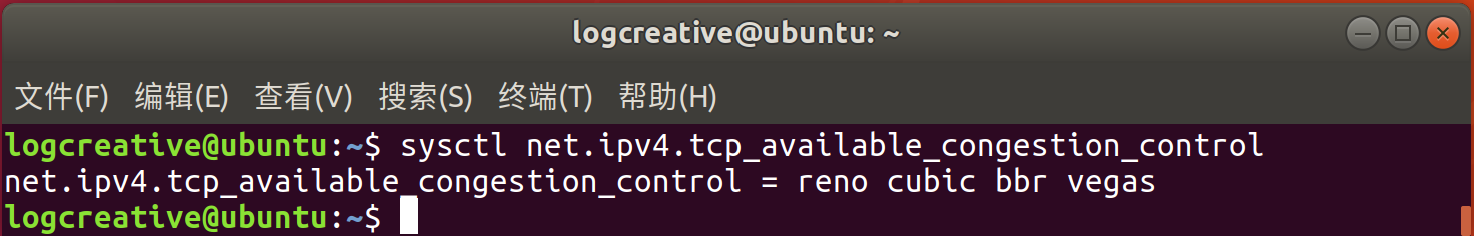
\includegraphics[width=\linewidth]{enable}
        \caption{开启TCP拥塞控制算法}\label{fig:enable}
    \end{figure}

    \noindent
    \begin{minipage}{0.4\textwidth}
        \begin{figure}[H]
            \centering
            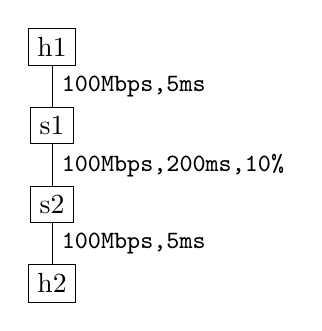
\begin{tikzpicture}
    \tikzstyle{host}=[draw]
    \tikzstyle{switch}=[draw]
    \tikzstyle{connection}=[]
    \tikzstyle{constr}=[right,font=\ttfamily\small]
    \node [host] (h1) at (0,4) {h1};
    \node [switch] (s1) at (0,3) {s1};
    \node [switch] (s2) at (0,2) {s2};
    \node [host] (h2) at (0,1) {h2};
    \draw (h1) edge node [constr] {100Mbps,5ms} (s1);
    \draw (s1) edge node [constr] {100Mbps,200ms,10\%} (s2);
    \draw (s2) edge node [constr] {100Mbps,5ms} (h2);
\end{tikzpicture}
            \caption{测试结构}\label{fig:task2topo}
        \end{figure}
        \begin{table}[H]
            \centering
            \caption{TCP 吞吐量(Mbps)}
            \pgfplotstabletypeset[columns/Alg/.style={string type}]{default.dat}
        \end{table}
    \end{minipage}
    \begin{minipage}{0.6\textwidth}
        \begin{figure}[H]
            \begin{tikzpicture}
                \begin{axis}[width=\linewidth,xlabel={Alg},
                ylabel={Throughput (Mbps)},
                ymin={0},
                symbolic x coords={reno,vegas}, xtick=data,
                ybar,enlarge x limits=0.8,]
                 \addplot+ [] table[x=Alg,y=Throughput,] {default.dat};
                \end{axis}
            \end{tikzpicture}
            \caption{TCP 吞吐量}
        \end{figure}
    \end{minipage}

    首先开启 TCP 拥塞控制算法 TCP Vegas,见图 \ref{fig:enable}。之后对两种算法进行测试,架构如图 \ref{fig:task2topo},测试代码见\href{./task2.py}{\ttfamily task2.py}。

    \section{多因素分析}
    Construct a network with only one pair of sender and receiver. Study how TCP throughput varies with respect to link bandwidth/link delay/loss rate for the above two TCP versions.

   本节测试的目的是为了对拥塞进行分析,所以对于\textbf{两个交换机之间的连接}进行单变量限制,默认值为 100 Mbps,无延迟无丢包,以查看相关结果。测试代码见 \href{./task3.py}{\ttfamily task3.py}。

   \begin{figure}[H]
       \centering
       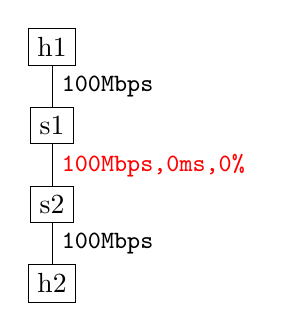
\begin{tikzpicture}
    \tikzstyle{host}=[draw]
    \tikzstyle{switch}=[draw]
    \tikzstyle{connection}=[]
    \tikzstyle{constr}=[right,font=\ttfamily\small]
    \node [host] (h1) at (0,4) {h1};
    \node [switch] (s1) at (0,3) {s1};
    \node [switch] (s2) at (0,2) {s2};
    \node [host] (h2) at (0,1) {h2};
    \draw (h1) edge node [constr] {100Mbps} (s1);
    \draw (s1) edge node [constr] {\color{red} 100Mbps,0ms,0\%} (s2);
    \draw (s2) edge node [constr] {100Mbps} (h2);
\end{tikzpicture}
       \caption{拓扑结构}\label{fig:task3topo}
   \end{figure}

    \subsection{带宽}

    带宽进行[20,180]Mbps 测试,每 10 Mbps 分为一个间隔。吞吐量随着带宽的增加几乎是正相关增长的,达到瓶颈后略有波动。其中 Reno 的带宽整体较高。

   \begin{figure}[H]
       \centering
       \begin{tikzpicture}
        \begin{axis}[xmin=0,ymin=0,ylabel={TCP Throughput (Mbps)},xlabel={Bandwidth (Mbps)},legend pos={south east}]
         \pgfplotstableread [] {bandwidth.dat}{\bw};
         \addplot+ [] table[x=bandwidth,y=reno,] {\bw};
         \addplot+ [] table[x=bandwidth,y=vegas,] {\bw};
         \legend{reno,vegas}
        \end{axis}
    \end{tikzpicture}
       \caption{带宽测试}\label{fig:bandwidth}
   \end{figure}

    \subsection{延迟}

    延迟进行[0,400]ms 测试,每 40 ms 分一个间隔。随着延迟的增长,吞吐量整体下降,Vegas 应对延迟性能较好。

   \begin{figure}[H]
       \centering
       \begin{tikzpicture}
        \begin{axis}[xmin=0,ymin=0,ymax=20,ylabel={TCP Throughput (Mbps)},xlabel={Delay (ms)}]
         \pgfplotstableread [] {delay.dat}{\delay};
         \addplot+ [] table[x=delay,y=reno,] {\delay};
         \addplot+ [] table[x=delay,y=vegas,] {\delay};
         \legend{reno,vegas}
        \end{axis}
    \end{tikzpicture}
       \caption{延迟测试}\label{fig:delay}
   \end{figure}

    \subsection{丢包}

    丢包进行[0,60]\% 测试,每 5\% 分一个间隔。丢包率增加对吞吐量变化几乎没有什么太大影响。Reno 较好。

   \begin{figure}[H]
       \centering
       \begin{tikzpicture}
        \begin{axis}[xmin=0,ymin=0,ylabel={TCP Throughput (Mbps)},xlabel={Loss (\%)},legend pos={south east}]
         \pgfplotstableread [] {loss.dat}{\loss};
         \addplot+ [] table[x=loss,y=reno,] {\loss};
         \addplot+ [] table[x=loss,y=vegas,] {\loss};
         \legend{reno,vegas}
        \end{axis}
    \end{tikzpicture}
       \caption{丢包测试}\label{fig:loss}
   \end{figure}

    \section{多机分析}

    Construct a network with a bottleneck link shared by multiple pairs of senders and receivers. Study how these sender-receiver pairs share the bottleneck link.

    由于 iPerf 不支持服务器并发服务,所以不能通过这种基准工具的方法进行测试。将采用 Socket Programming 实验中的 C/S 模型软件进行测试。

    采用如图 \ref{fig:task4topo} 类似的树状结构,中间会有一个瓶颈 45Mbps 的线路,每一个客户端会分配到 $25\frac{i}{n}$ Mbps 的带宽。
    % 当 $n = 5$ 时,
    客户端分配的带宽如表 \ref{tab:bandwidth}。框架实现代码见 \href{./task4.py}{\ttfamily task4.py}。

    \noindent
    \begin{minipage}{0.5\textwidth}
        \begin{figure}[H]
            \centering
            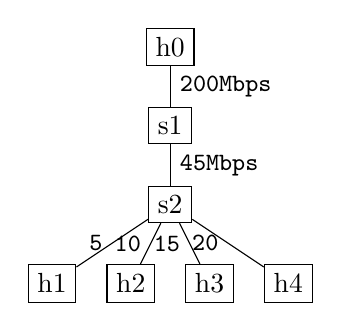
\begin{tikzpicture}
    \tikzstyle{host}=[draw]
    \tikzstyle{switch}=[draw]
    \tikzstyle{connection}=[]
    \tikzstyle{constr}=[right,font=\ttfamily\small]
    \node [host] (h0) at (0,4) {h0};
    \node [switch] (s1) at (0,3) {s1};
    \node [switch] (s2) at (0,2) {s2};
    \node [host] (h2) at (-0.5,1) {h2};
    \draw (h0) edge node [constr] {200Mbps} (s1);
    \draw (s1) edge node [constr] {45Mbps} (s2);
    \draw (s2) edge node [constr,left] {10} (h2);
	\node[host] (v1) at (-1.5,1) {h1};
	\node[host] (v2) at (0.5,1) {h3};
\draw  (s2) edge node [constr,left] {5} (v1);
\draw  (s2) edge node [constr,left] {15} (v2);
\node [host] (v3) at (1.5,1) {h4};
\draw  (s2) edge node [constr,left] {20} (v3);
\end{tikzpicture}
            \caption{拓扑结构}\label{fig:task4topo}
        \end{figure}
    \end{minipage}
    \begin{minipage}{0.5\textwidth}
        \begin{table}[H]
        \centering
        \caption{分配带宽($n=5$)}\label{tab:bandwidth}
        \begin{tabular}{ccccc}
            \toprule
                & h1 & h2 & h3 & h4\\
            \midrule
            带宽(Mbps) & 5 & 10 & 15 & 20 \\
            \bottomrule
        \end{tabular}
    \end{table}
    \end{minipage}
    \vspace*{5pt}
    
    \begin{figure}[H]
        \centering
        \begin{minipage}{0.48\textwidth}
            \centering
            \begin{tikzpicture}
                \begin{axis}[symbolic x coords={h1,h2,h3,h4}, xtick=data,
                ybar,ylabel={TCP Throughput (Mbps)},xlabel={Client},width=\linewidth,legend pos=north west]
                 \addplot+ [] table[x=Host,y=Speed,] {reno_multi.dat};
                 \pgfplotsset{cycle list shift=1};
                 \addplot+ [] coordinates { (h1,5) (h2,10) (h3,15) (h4,20)};
                \legend{Reno,Limit}
                \end{axis}
                \end{tikzpicture}                
            \caption{Reno 多机测试}\label{fig:renom}
        \end{minipage}
        \begin{minipage}{0.48\textwidth}
            \centering
            \begin{tikzpicture}
                \begin{axis}[symbolic x coords={h1,h2,h3,h4}, xtick=data,
                ybar,xlabel={Client},width=\linewidth,legend pos=north west]
                \pgfplotsset{cycle list shift=1};
                 \addplot+ [] table[x=Host,y=Speed,] {vegas_multi.dat};
                 \addplot+ [] coordinates { (h1,5) (h2,10) (h3,15) (h4,20)};
                 \legend{Vegas,Limit}
                \end{axis}
                \end{tikzpicture}   
            \caption{Vegas 多机测试}\label{fig:vegasm}
        \end{minipage}
    \end{figure}

    图 \ref{fig:renom} 显示了 Reno 对于带宽分配上更加接近 Max-Min Fairness,整体带宽为 40Mbps。而图 \ref{fig:vegasm} 显示 Vegas 更倾向于高带宽给高速度,提高了总体的带宽利用率(43Mbps)。


\end{document}